\begin{frame}{Composable Data Structures}
  \begin{center}
    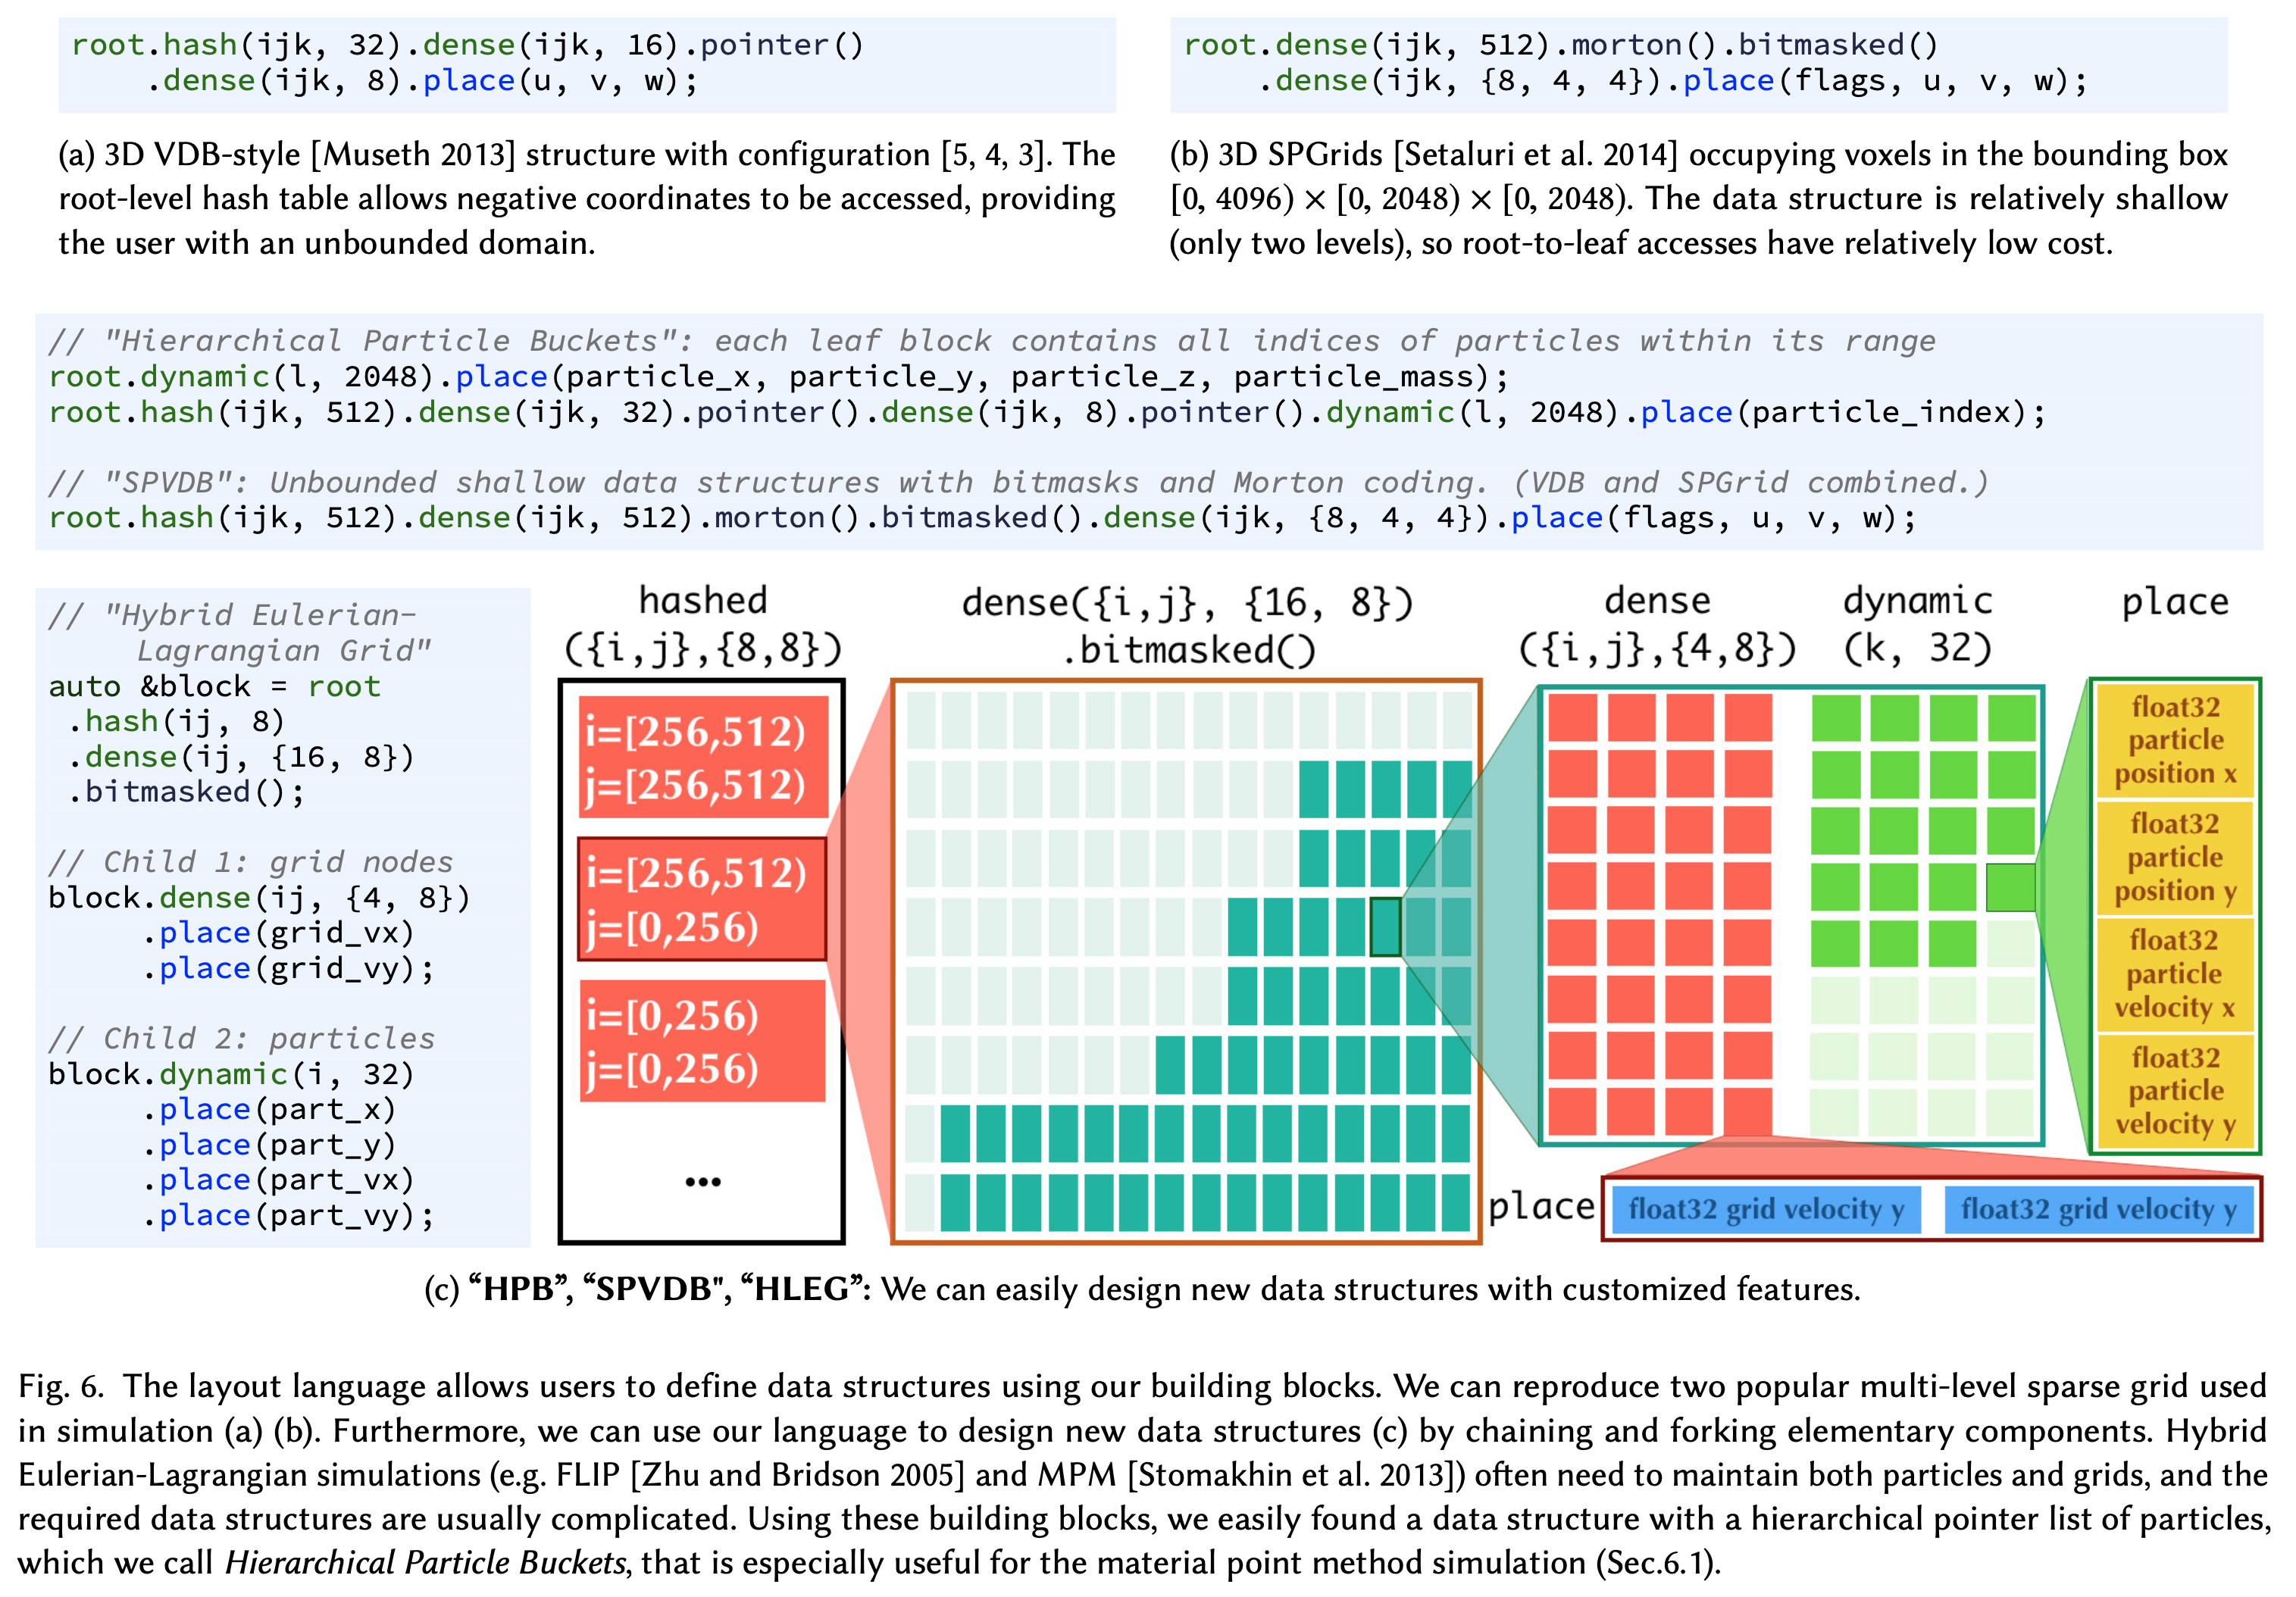
\includegraphics[width=10cm]{taichi_data_structures.png}
    \blfootnote{From \cite{Hu2019}}
  \end{center}
\end{frame}

\begin{frame}{Objective Data-oriented Programming Example}
  \begin{center}
    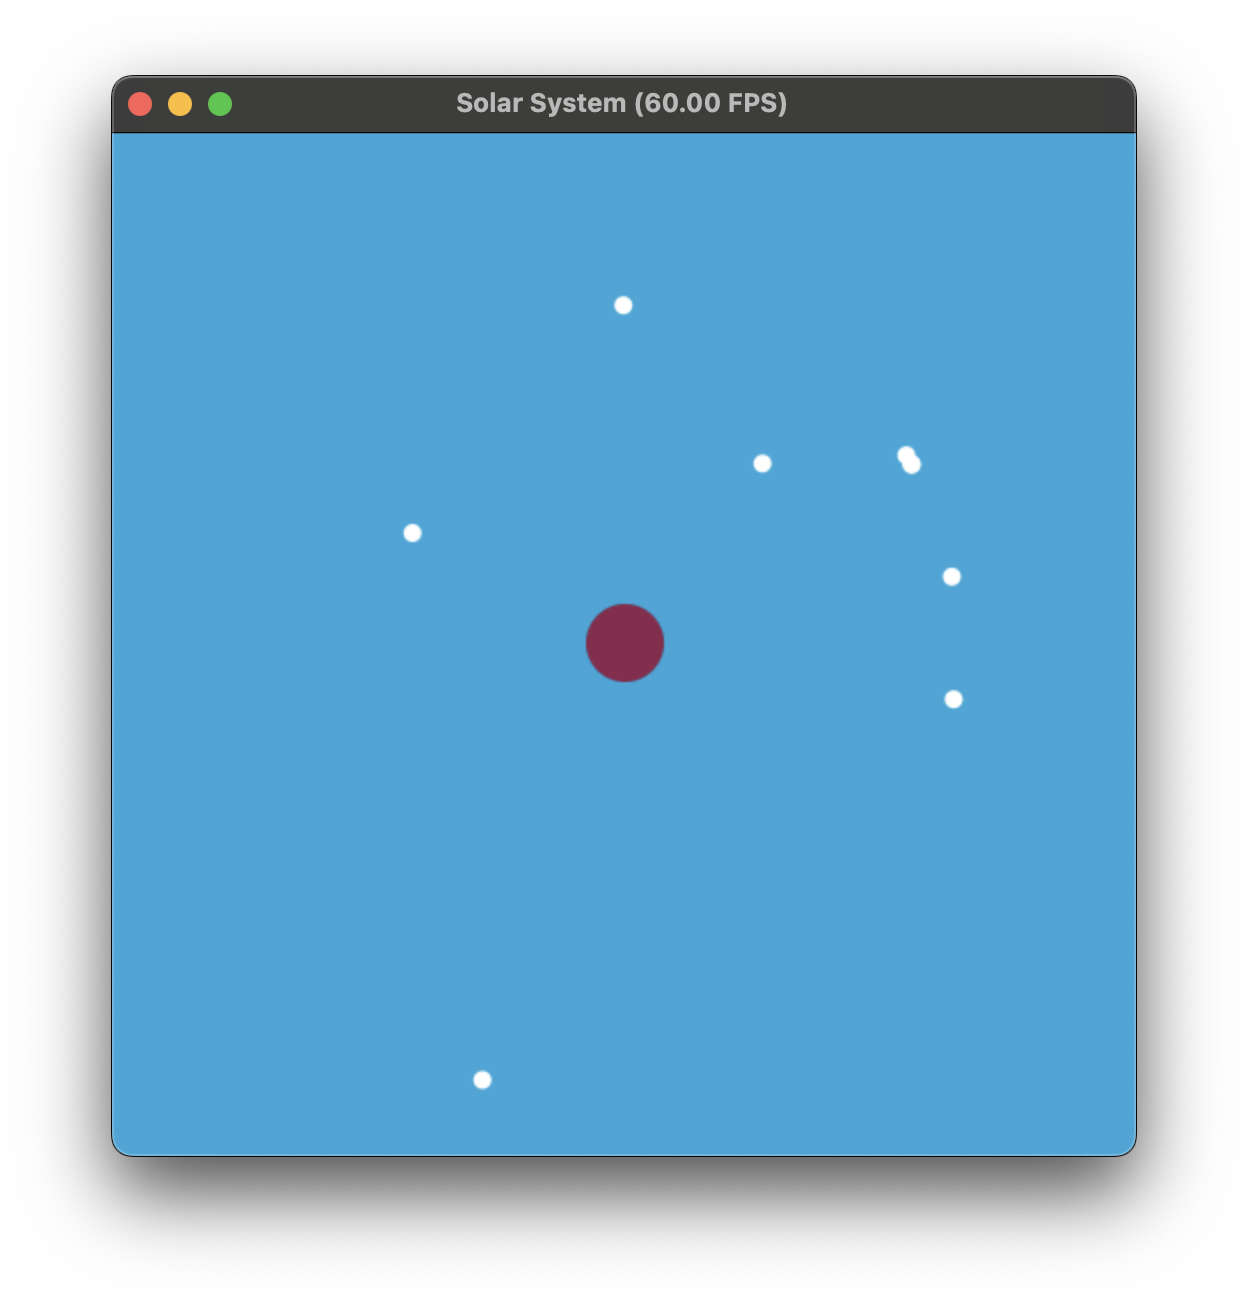
\includegraphics[width=6cm]{data_oriented_example.png}
    \blfootnote{Adapted from \href{https://yuanming.taichi.graphics/publication/2020-taichi-tutorial/taichi-tutorial.pdf}{Taichi SIGGRAPH Workshop} slides}
  \end{center}
\end{frame}

\begin{frame}{Physical Simulation Example}
\begin{columns}
  \column{0.48\linewidth}
  \begin{center}
    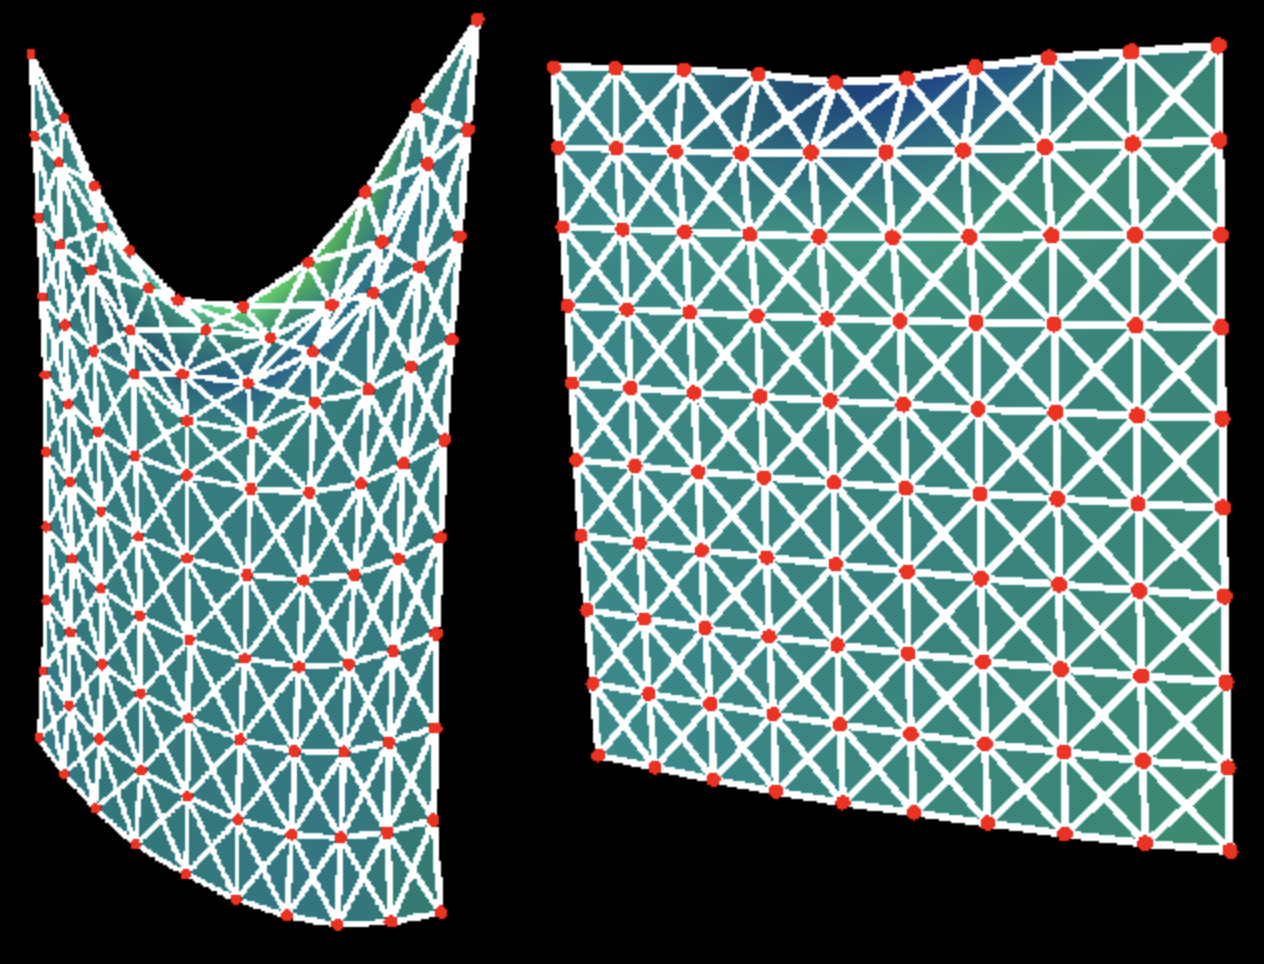
\includegraphics[width=3cm]{cloth_mesh.png}\\
    \vspace{0.5cm}
    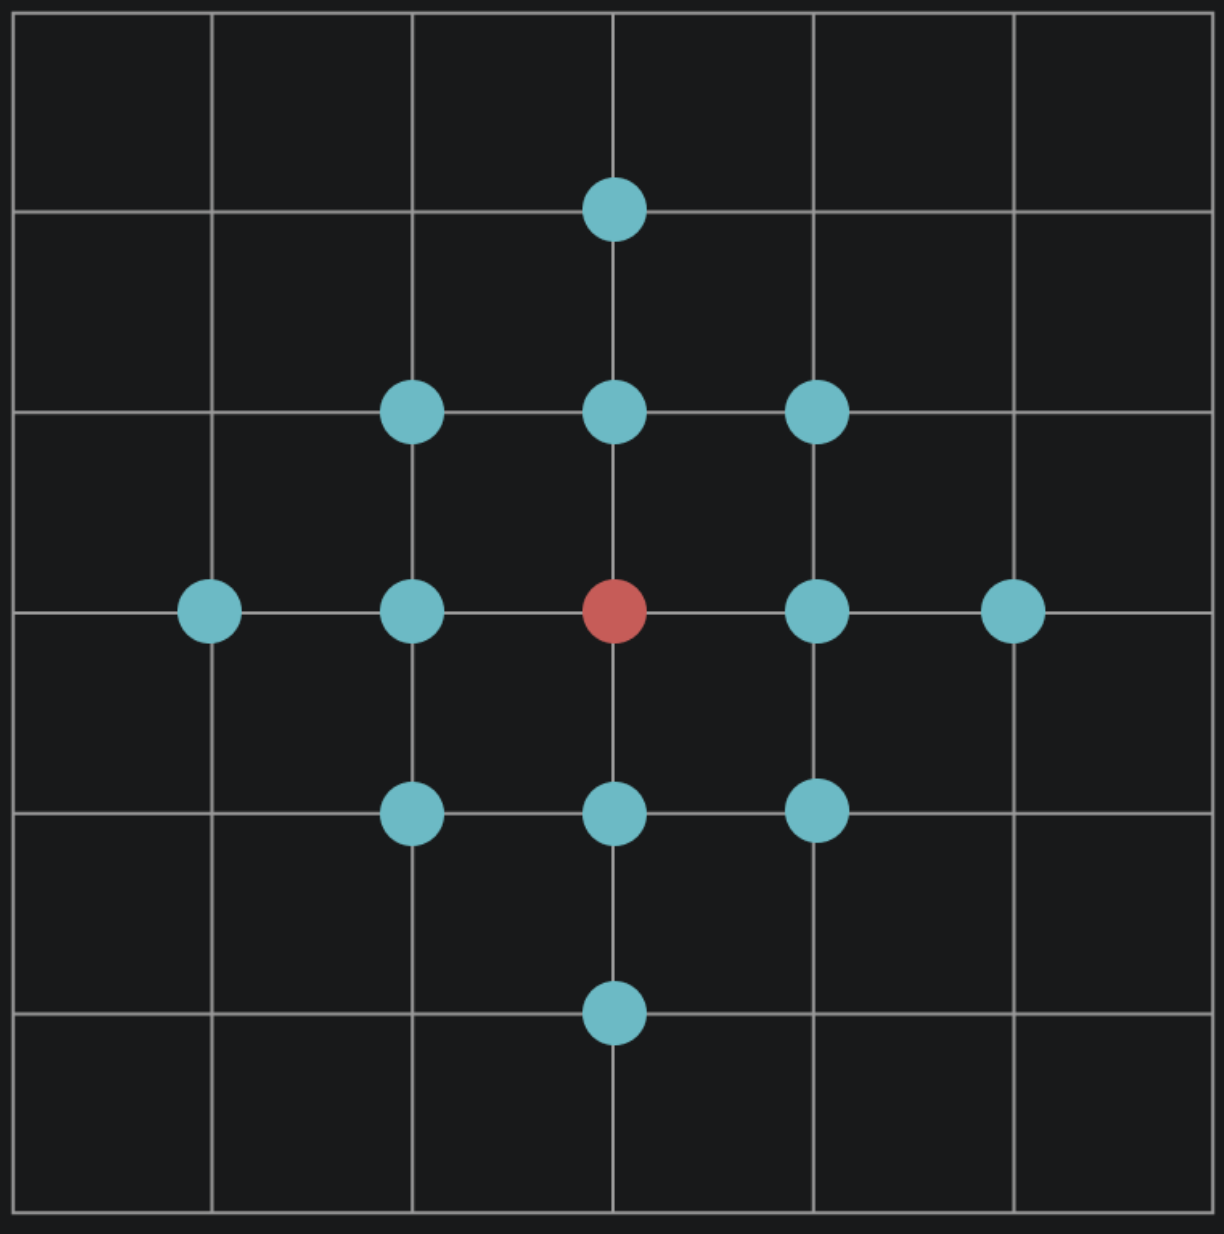
\includegraphics[width=3cm]{spring_stencil.png}
  \end{center}

  \column{0.48\linewidth}
  \centering
  \begin{center}
    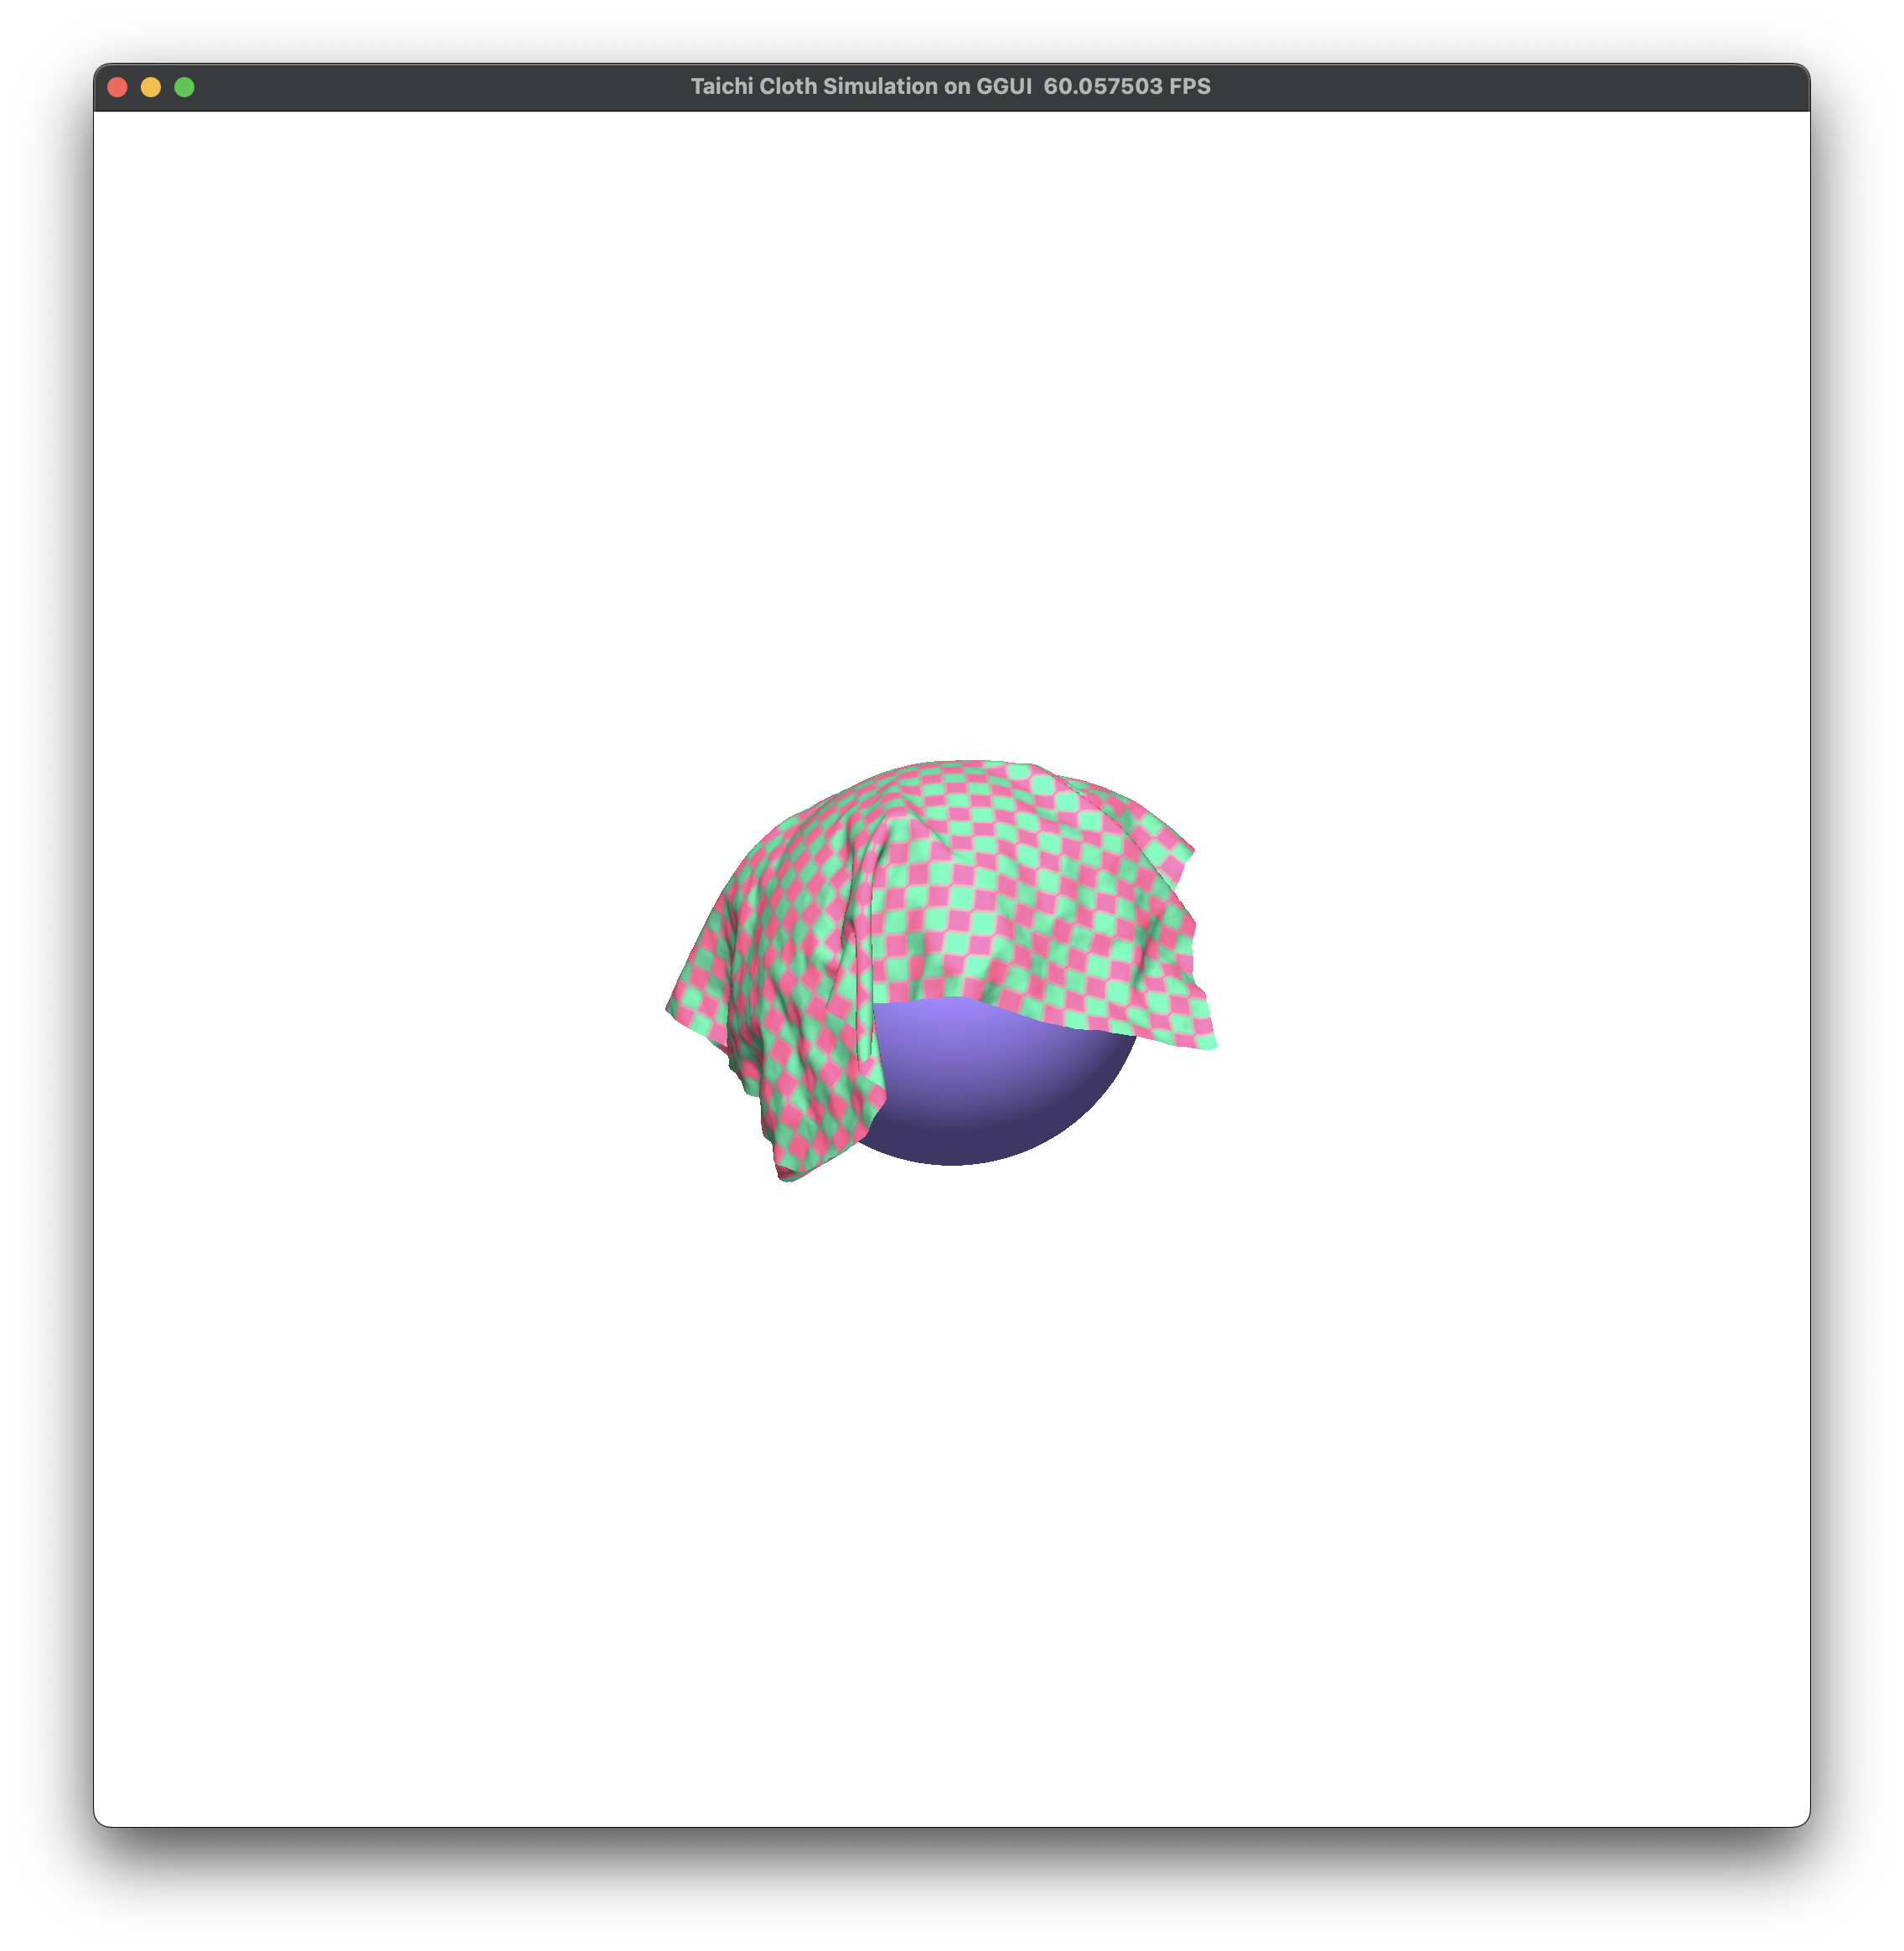
\includegraphics[width=5cm]{cloth_example.png}
  \end{center}
\end{columns}
\blfootnote{Adapted from \href{https://docs.taichi-lang.org/docs/cloth_simulation}{Conduct Physical Simulation} guide}
\end{frame}




